



\documentclass[conference,compsoc]{IEEEtran}




% *** CITATION PACKAGES ***
%
\ifCLASSOPTIONcompsoc
  % IEEE Computer Society needs nocompress option
  % requires cite.sty v4.0 or later (November 2003)
  \usepackage[nocompress]{cite}
\else
  % normal IEEE
  \usepackage{cite}
\fi





% *** GRAPHICS RELATED PACKAGES ***
%
\ifCLASSINFOpdf
  % \usepackage[pdftex]{graphicx}
  % declare the path(s) where your graphic files are
  % \graphicspath{{../pdf/}{../jpeg/}}
  % and their extensions so you won't have to specify these with
  % every instance of \includegraphics
  % \DeclareGraphicsExtensions{.pdf,.jpeg,.png}
\else
  % or other class option (dvipsone, dvipdf, if not using dvips). graphicx
  % will default to the driver specified in the system graphics.cfg if no
  % driver is specified.
  % \usepackage[dvips]{graphicx}
  % declare the path(s) where your graphic files are
  % \graphicspath{{../eps/}}
  % and their extensions so you won't have to specify these with
  % every instance of \includegraphics
  % \DeclareGraphicsExtensions{.eps}
\fi





% *** MATH PACKAGES ***
%

\usepackage[fleqn]{amsmath}
\usepackage{amsmath, amsthm, amsfonts}
\usepackage{amsmath}

% A popular package from the American Mathematical Society that provides
% many useful and powerful commands for dealing with mathematics.
%
% Note that the amsmath package sets \interdisplaylinepenalty to 10000
% thus preventing page breaks from occurring within multiline equations. Use:
%\interdisplaylinepenalty=2500
% after loading amsmath to restore such page breaks as IEEEtran.cls normally
% does. amsmath.sty is already installed on most LaTeX systems. The latest
% version and documentation can be obtained at:
% http://www.ctan.org/pkg/amsmath





% *** SPECIALIZED LIST PACKAGES ***
\usepackage{hyperref}
\usepackage[margin=1in]{geometry}
\usepackage{graphicx}
\usepackage{caption}
\usepackage{subcaption}
\usepackage{float}
\newcommand{\vertSpace}[1]{\vspace{3mm}}




% *** ALIGNMENT PACKAGES ***
%
%\usepackage{array}
% Frank Mittelbach's and David Carlisle's array.sty patches and improves
% the standard LaTeX2e array and tabular environments to provide better
% appearance and additional user controls. As the default LaTeX2e table
% generation code is lacking to the point of almost being broken with
% respect to the quality of the end results, all users are strongly
% advised to use an enhanced (at the very least that provided by array.sty)
% set of table tools. array.sty is already installed on most systems. The
% latest version and documentation can be obtained at:
% http://www.ctan.org/pkg/array


% IEEEtran contains the IEEEeqnarray family of commands that can be used to
% generate multiline equations as well as matrices, tables, etc., of high
% quality.




% *** SUBFIGURE PACKAGES ***
%\ifCLASSOPTIONcompsoc
%  \usepackage[caption=false,font=footnotesize,labelfont=sf,textfont=sf]{subfig}
%\else
%  \usepackage[caption=false,font=footnotesize]{subfig}
%\fi
% subfig.sty, written by Steven Douglas Cochran, is the modern replacement
% for subfigure.sty, the latter of which is no longer maintained and is
% incompatible with some LaTeX packages including fixltx2e. However,
% subfig.sty requires and automatically loads Axel Sommerfeldt's caption.sty
% which will override IEEEtran.cls' handling of captions and this will result
% in non-IEEE style figure/table captions. To prevent this problem, be sure
% and invoke subfig.sty's "caption=false" package option (available since
% subfig.sty version 1.3, 2005/06/28) as this is will preserve IEEEtran.cls
% handling of captions.
% Note that the Computer Society format requires a sans serif font rather
% than the serif font used in traditional IEEE formatting and thus the need
% to invoke different subfig.sty package options depending on whether
% compsoc mode has been enabled.
%
% The latest version and documentation of subfig.sty can be obtained at:
% http://www.ctan.org/pkg/subfig




% *** FLOAT PACKAGES ***
%
%\usepackage{fixltx2e}
% fixltx2e, the successor to the earlier fix2col.sty, was written by
% Frank Mittelbach and David Carlisle. This package corrects a few problems
% in the LaTeX2e kernel, the most notable of which is that in current
% LaTeX2e releases, the ordering of single and double column floats is not
% guaranteed to be preserved. Thus, an unpatched LaTeX2e can allow a
% single column figure to be placed prior to an earlier double column
% figure.
% Be aware that LaTeX2e kernels dated 2015 and later have fixltx2e.sty's
% corrections already built into the system in which case a warning will
% be issued if an attempt is made to load fixltx2e.sty as it is no longer
% needed.
% The latest version and documentation can be found at:
% http://www.ctan.org/pkg/fixltx2e


%\usepackage{stfloats}
% stfloats.sty was written by Sigitas Tolusis. This package gives LaTeX2e
% the ability to do double column floats at the bottom of the page as well
% as the top. (e.g., "\begin{figure*}[!b]" is not normally possible in
% LaTeX2e). It also provides a command:
%\fnbelowfloat
% to enable the placement of footnotes below bottom floats (the standard
% LaTeX2e kernel puts them above bottom floats). This is an invasive package
% which rewrites many portions of the LaTeX2e float routines. It may not work
% with other packages that modify the LaTeX2e float routines. The latest
% version and documentation can be obtained at:
% http://www.ctan.org/pkg/stfloats
% Do not use the stfloats baselinefloat ability as the IEEE does not allow
% \baselineskip to stretch. Authors submitting work to the IEEE should note
% that the IEEE rarely uses double column equations and that authors should try
% to avoid such use. Do not be tempted to use the cuted.sty or midfloat.sty
% packages (also by Sigitas Tolusis) as the IEEE does not format its papers in
% such ways.
% Do not attempt to use stfloats with fixltx2e as they are incompatible.
% Instead, use Morten Hogholm'a dblfloatfix which combines the features
% of both fixltx2e and stfloats:
%
% \usepackage{dblfloatfix}
% The latest version can be found at:
% http://www.ctan.org/pkg/dblfloatfix




% *** PDF, URL AND HYPERLINK PACKAGES ***
%
%\usepackage{url}
% url.sty was written by Donald Arseneau. It provides better support for
% handling and breaking URLs. url.sty is already installed on most LaTeX
% systems. The latest version and documentation can be obtained at:
% http://www.ctan.org/pkg/url
% Basically, \url{my_url_here}.




% *** Do not adjust lengths that control margins, column widths, etc. ***
% *** Do not use packages that alter fonts (such as pslatex).         ***
% There should be no need to do such things with IEEEtran.cls V1.6 and later.
% (Unless specifically asked to do so by the journal or conference you plan
% to submit to, of course. )


% correct bad hyphenation here
\hyphenation{op-tical net-works semi-conduc-tor}


\begin{document}
%
% paper title
% Titles are generally capitalized except for words such as a, an, and, as,
% at, but, by, for, in, nor, of, on, or, the, to and up, which are usually
% not capitalized unless they are the first or last word of the title.
% Linebreaks \\ can be used within to get better formatting as desired.
% Do not put math or special symbols in the title.
\title{Exploring Loan Discrimination with Big Data}


% author names and affiliations
% use a multiple column layout for up to three different
% affiliations
\author{
      Cody Gilbert \\
        NYU Computer Science \\
        New York, USA \\
        cjg507@nyu.edu \\
            \and
        Fang Han\\
        NYU Computer Science \\
        New York, USA \\
        fh643@nyu.edu\\
             \and
        Jeremy Lao \\
        NYU Computer Science  \\
        Washington, USA \\
        jjl359@nyu.edu



}




% make the title area
\maketitle

% As a general rule, do not put math, special symbols or citations
% in the abstract
\begin{abstract}
The objective of this analysis is to draw actionable and insightful analysis regarding US loan approval bias using the Home Mortgage Disclosure Act (HMDA) data between 2007-2017, and to create an application for determining biases in lender practices. The tool was constructed using the Apache Spark framework to analyze and process data, with the MLLib package used to construct a model for predicting loan approval given loan applicant demographics. The model will produce an output that feeds a user interface (UI) to display a summary of what lenders are most likely to approve a loan given the user's input demographics. The final model used a Naive Bayes model with a poor predictive quality of 80% AUC-ROC, but could not be improved due to time constraints.  


\end{abstract}

% no keywords
\begin{keywords}
mortgage, HMDA, Naive Bayes, fair lending, logistic regression, loans
\end{keywords}

% For peer review papers, you can put extra information on the cover
% page as needed:
% \ifCLASSOPTIONpeerreview
% \begin{center} \bfseries EDICS Category: 3-BBND \end{center}
% \fi
%
% For peerreview papers, this IEEEtran command inserts a page break and
% creates the second title. It will be ignored for other modes.
\IEEEpeerreviewmaketitle



\section{Introduction}

In the ongoing struggle and debate over civil rights within the United States, the notion of equality in the delivery of essential services to persons of all races, genders, and ethnicities is considered an essential element to a free and productive nation. Housing, and the services to own and lease property, are  critically important elements of these essential services that have had a tumultuous recorded history of discrimination within the US. To combat the loan inequality that hurt minority populations, US Congress enacted the 1975 Home Mortgage Disclosure Act (HMDA) that required lending institutions to supply loan data to the US Federal Government with the goal of identifying possible discriminatory lending patterns among lenders.  To put it in plainly, if someone applies for a mortgage related loan, that data point and the anonymized metadata of the applicant are reported to the Consumer Financial Protection Bureau (CFPB). 
The objective of this analysis is use this HMDA data to create a user-interactive tool for discovering biases and trends in US lending practices. This tool will allow users to select a set of demographics to see how differences in race, ethnicity, and gender impact the chances of having a loan approved, how those chances have changed over time, and what institutions show the highest levels of bias. The goal of this project to provide potential lenders information on what lending institutions best fit their needs, and contribute an additional resource to the ongoing discussion of inequality within the United States.

\section{Motivation}

The Home Mortgage Disclosure Act (HMDA) dataset is one of the largest publicly available datasets in banking with application and demographic level data.  While the banking regulators have used the dataset to monitor the mortgage market and unfair lending practices for many years, it is also important for the public to understand the dataset.  The application that we are proposing is just one tool that can help the public utilize the publicly available information in choosing a lender when applying for a loan.  The machine learning methods can help a loan applicant identify a lender that has the highest probability of lending to the applicant using the applicant’s metadata.  


\section{Related Work}

Previous research on this topic are primarily based on the regulator’s perspective.  For example, in \cite{FDIC} the banking regulators outlined the process by which they conduct investigations into unfair lending practices using the HMDA dataset as a starting point.  The Federal Reserve and the FDIC both use the dataset to monitor and enforce both the community reinvestment act and fair lending practices. 
The Federal Reserve publishes analysis performed on the HMDA dataset, and have highlighted both the rich analysis that can be obtained from the data along with the shortcomings of the dataset.  For example, in \cite{FED} Federal Reserve economists highlight the importance of modeling and controlling for various loan application characteristics when interpreting the denial rate of a loan application by race and gender. 
Current regulatory research on the topic shows that the HMDA dataset contains valuable insight that can be analyzed and modeled to reveal patterns of discriminatory behavior. It is this insight that motivates the construction of the tool created in this project.

\section{Datasets}


\subsection{Home Mortgage Disclosure Act}
he Home Mortgage Disclosure Act (HMDA) was originally enacted by Congress in 1975 and is implemented by Regulation C. This regulation applies to certain financial institutions, including banks, savings associations, credit unions, and other mortgage lending institutions.  HMDA requires many financial institutions to maintain, report, and publicly disclose loan-level information about mortgages. These data help show whether lenders are serving the housing needs of their communities. They give public officials information that helps them make decisions and policies, and they shed light on lending patterns that could be discriminatory. The public data are modified to protect applicant and borrower privacy. The data available for public use is summarized in Table 1.

\begin{table}[h!]
\centering
\begin{tabular}{|c|c|c|c|}
\hline
\textbf{Year} & \textbf{Activity Year} & \textbf{No. Reporters} & \textbf{No. Records  (mm)} \\ \hline
2017           & 2016               & 6,762                      & 16.3                                    \\ \hline
2016           & 2015               & 6,913                      & 14.3                                    \\ \hline
2015           & 2014               & 7,062                      & 11.9                                    \\ \hline
2014           & 2013               & 7,190                      & 17                                      \\ \hline
2013           & 2012               & 7,400                      & 18.7                                    \\ \hline
2012           & 2011               & 7,632                      & 14.7                                    \\ \hline
2011           & 2010               & 7,923                      & 16.3                                    \\ \hline
2010           & 2009               & 8,124                      & 19.5                                    \\ \hline
2009           & 2008               & 8,388                      & 17.4                                    \\ \hline
2008           & 2007               & 8,610                      & 26.6                                    \\ \hline
2007           & 2006               & 8,886                      & 34.1                                   \\ \hline
\end{tabular}
\caption{HMDA Data Summary}
\end{table}

\subsection{Nationwide Institution Data}
In close relation to the HMDA data, the nationwide institution data is a series of fixed format flat files of all lending institutions that reported HMDA data from 2007 to 2017. These files come in two different schemas, offering information regarding the lending institution, its parent institution and its top holder, including ID, name, and state. 

\subsection{Mapping Data}

Data was acquired to validate the geographic distribution of HMDA data as well as provide enhanced visualizations within the output tool. The data used to map the geography of the loan data was taken from two source files for US County \cite{USCensusOne} and US State \cite{USCensusTwo} geometry data. The geometry data was compiled by the US Census Bureau as a collection of TIGER/Line shapefiles and related database files. These files are extracts of selected geographic and cartographic information from the U.S. Census Bureau's Master Address File / Topologically Integrated Geographic Encoding and Referencing (MAF/TIGER) Database (MTDB). 


\section{Description of Analytic}

The core principle of operation of this analysis and resulting application is the use of machine learning to create a supervised machine learning classification model to determine the probability of loan application approval. The user of the tool will enter their demographic information (e.g. US State, income, Race, etc.) which will be processed by the model to produce a probability of loan approval by historical year and lender. This model will effectively condense the 100+ million rows of HMDA and allow users to query acceptance rates for their particular cohort. 


    The input features for the model were chosen based on features both present in the HMDA dataset and considered relevant for loan application approval prediction. The following features are included in the model:


\begin{enumerate}
\item Applicant Race
\item Applicant Ethnicity
\item Applicant Gender
\item Applicant Income
\item Loan Amount
\item Respondent ID (Lender ID)
\item Year of Application
\item State of application


\end{enumerate}

The classification outcome was a binary “Approved” or “Denied” status. The output used for the final visualization will be the model’s probability of approval, which is typically bucketed into a binary classification by some threshold value. The model was fit to the HMDA data based on these features to create a predictive model for use in the application.

Users of the application will enter their demographic and loan application information, which will be fed into the features described above. A pre-populated table of lenders and application years will be created and the cartesian product of lender, year, and user provided information will be input to the model. The model output will result in a probability of approval for each year and lender for the given demographics.

The table of loan approval probabilities will be presented to the user using visualization tools within a Flask web application. The user will then be able to repeat the submission process for different values to compare loan approval distributions.   

\section{Application Design}

The design process used to generate the output loan bias visualization tool followed the data flow shown in Figure 1.


\begin{figure}[h!]
  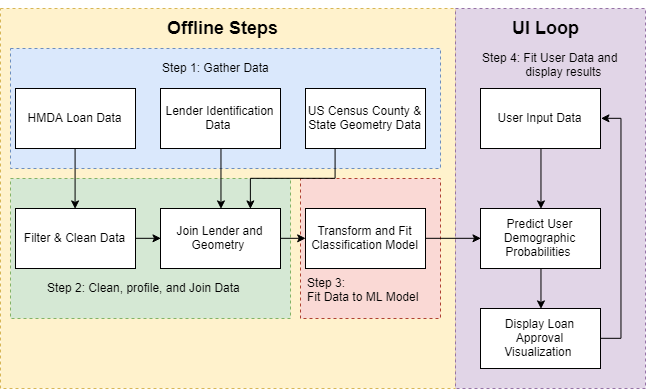
\includegraphics[width=\linewidth]{SparkDesignDiagram.png}
  \caption{Design Data Flow Diagram}
  \label{fig:design}
\end{figure}


The design supports the following data flow steps:
\begin{enumerate}

\item HMDA data, lender identification data, and US Census geography data were downloaded and stored within the NYU Dumbo Hadoop cluster.

\item Spark was used to clean, profile, and filter the data sets. Each data set was joined to create a table containing all pertinent user demographic data.

\item HMDA features were selected, transformed, and fit to a logistic regression model. The model was saved to file for fast online access.

\item An application was created to support the loan bias visualization tool flow loop:

\begin{enumerate}
\item User inputs demographic and loan application information
\item Input information is transformed and the saved model is used to calculate a dataframe of loan approval probabilities
\item The predicted data is shown to the user, who can input new information to iterate the loop
\end{enumerate}

\end{enumerate}


\section{Actuation or Remediation}

 The end result of this project is a tool intended for use by potential loan applicants, equal housing advocates, and US financial regulatory policymakers to discern potential discriminatory patterns in lending and take appropriate actions. A potential loan applicant may enter their information and decide what lenders should be pursued or avoided for their demographic. Advocates and policymakers can iterate upon the results of the tool to determine the differences in lender behavior related to protected classes and take further regulatory action.

\section{Analysis}

\subsection{HMDA Data}

The HMDA data, the primary data source for this analysis, was uploaded to the NYU Dumbo Hadoop cluster and placed within HDFS.  The data was extensively profiled in order to understand data quality, underlying distribution of some continuous variables, and understand each data fields’ values to determine which fields should be used in the machine learning model.  The time period that this dataset covers is from 2007-2017. 

	HMDA data is collected by the Consumer Financial Protection Bureau (CFPB) and made available to the public on their website \cite{hmdalink}.  The data were ingested into NYU’s scratch folder using a bash script of curl commands that downloaded the zip file and subsequently unzipped the file into scratch and subsequently loaded to HDFS.  The HMDA dataset comes in two versions.  
The first version is a ‘raw’ dataset that represents the respondents (lending institutions) categorical (i.e. textual information) as categorical variables and continuous variables as a string of integers.  For example, the respondent represents the gender of the loan applicant as ‘1’ for male and ‘2’ for female.  The state and county are represented by their FIPS code (Federal Information Processing Standard).  

The second version is a complete textual representation of the loan applicant’s metadata.  For example, gender is represented as either ‘Male’ or ‘Female’ and the state and county are represented by the abbreviation and county name. 

Ultimately the size of the second version of the dataset is nearly twice as large as the ‘raw’ version.  While it is easier to deal with the full textual representation of the data, there was a considerable performance issue with ingesting and processing the dataset during the profiling stage.  The data set is provided as a CSV file by the CFPB.  However, in the textual representation of the HMDA data, some fields are long descriptions that include embedded commas.  Therefore, the only way that we found to process that dataset in Spark was by using a SQL context and ingesting the data as a ‘dataframe’.  However, with ~150 GB of data, the data profiling process would require six hours to complete.  

Due to the slow performance of data profiling the textual HMDA information the team decided to process the underlying ‘raw’ dataset using the spark context resilient distributed dataset (RDD) abstraction.  While there was a significant amount of coding required to filter out empty strings and NA representations, along with considerable work to translate the categorical variable to the textual representation, the data profiling portion of the project was much quicker by a factor of 4x. 

We profiled the continuous variable, ‘loan application amount’ for the 2013 dataset, and we found that the frequency of loan application amounts look somewhat normally distributed between \$10,000 and \$500,000.  There is a very fat tail to the right (larger loan amounts).  In deciding which data we should model, we decided to filter for loan applications between \$50,000 and \$500,000 in order to have a normally distributed continuous variable.  Similarly we filtered for applicant income between \$25,000 and \$100,000 assuming there would be normal distribution of income frequencies in that range. 

\begin{figure}[h!]
  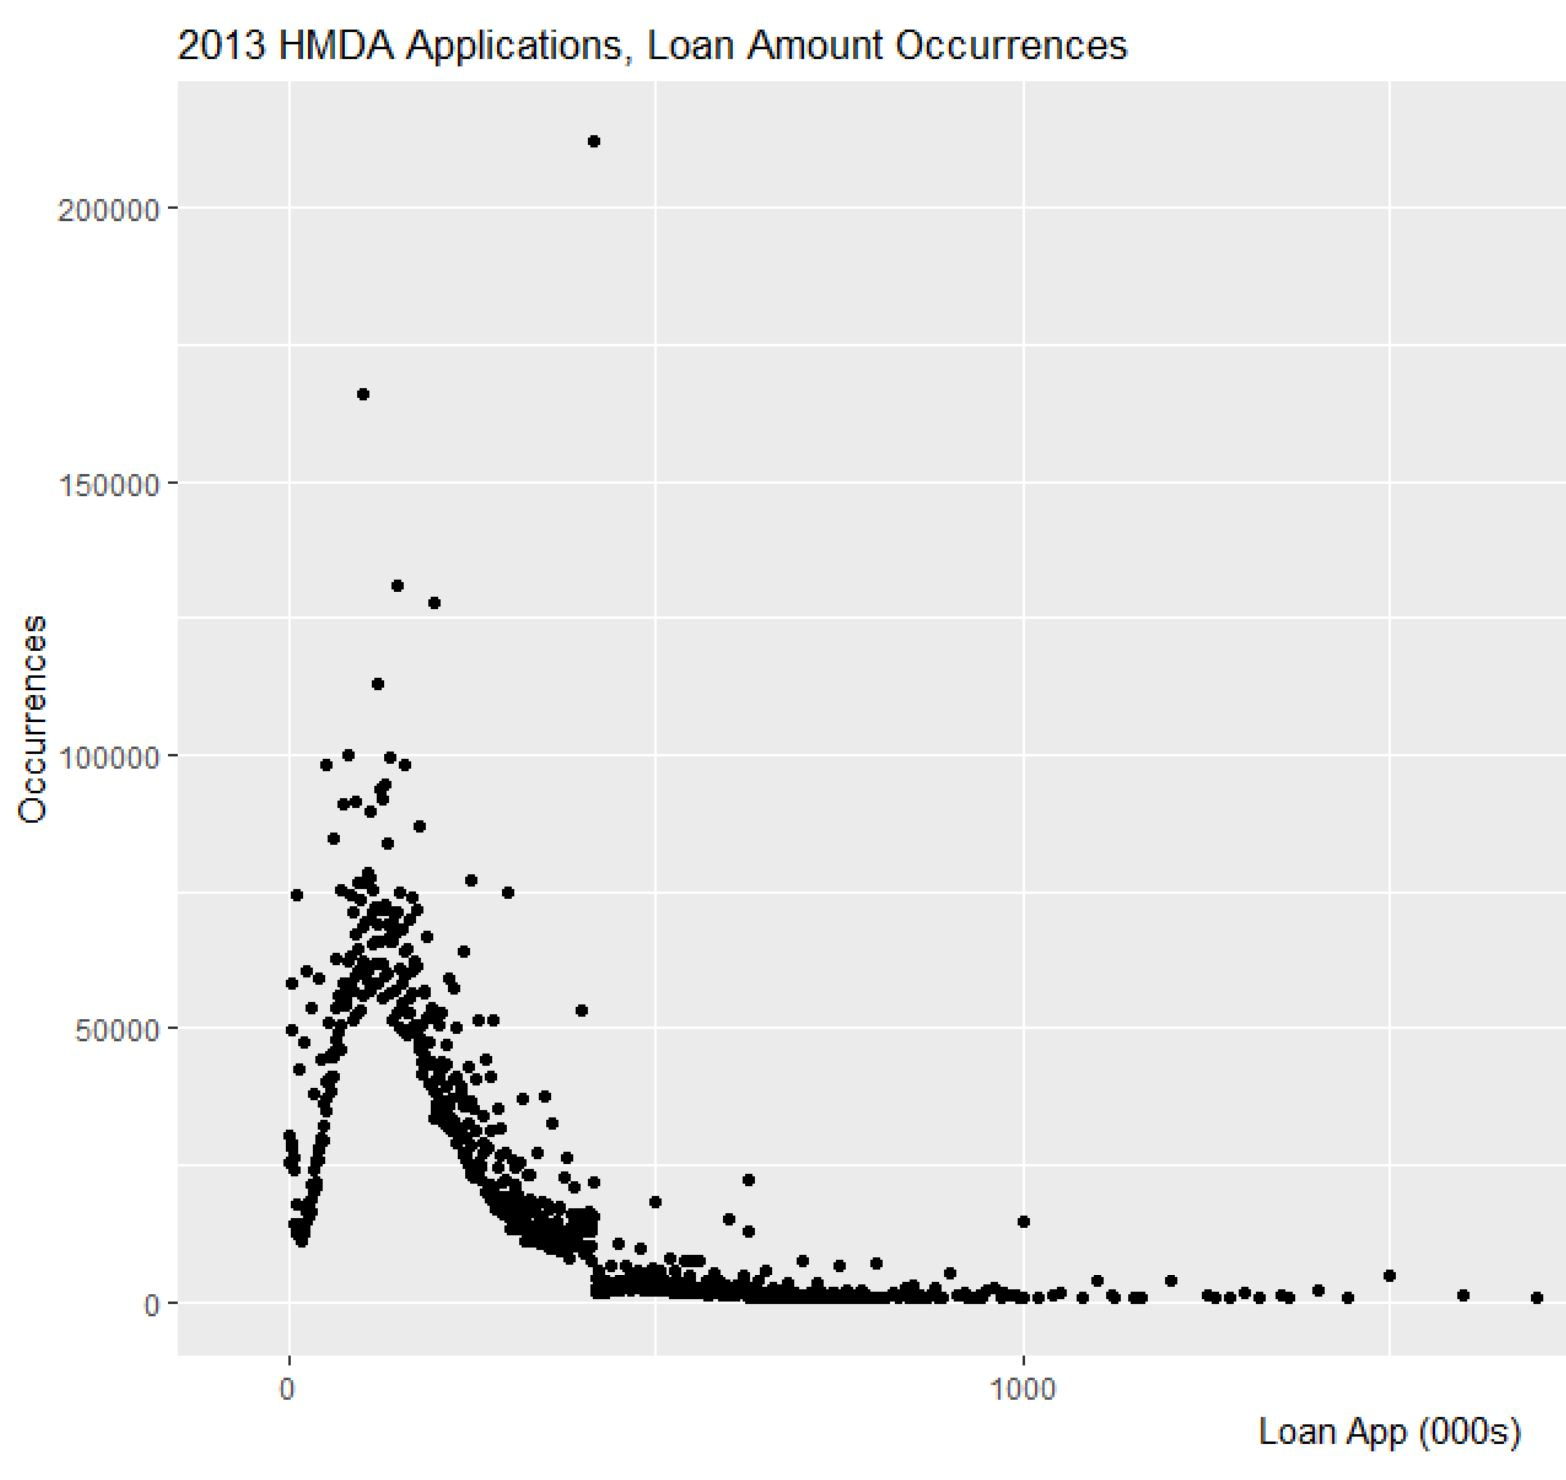
\includegraphics[width=\linewidth]{Loan_App_Dist.jpg}
  \caption{Loan App Frequency Distribution}
  \label{fig:design}
\end{figure}


\subsection{Nationwide Institution Data}

nder the Home Mortgage Disclosure Act (HMDA), financial institutions are required to report data about mortgages to the public, whose own information is in turn compiled into csv files and available from 2007 to 2017 by year. Compared to the millions of records in the HMDA data, the institution dataset is quite small, totaling no more than 30MB. Challenges, nevertheless, are still present from primarily these two aspects: 

\begin{enumerate}
\item Data recorded before and after 2010 used formats that are dramatically different, namely about a third of non-trivial fields were not recorded at all before 2010. 
\item We were hoping that “Respondent ID” could serve as the primary key to query into the dataset, in order to facilitate project actuation. However it turns out that not only are these IDs not unique, there’s no pairwise bijection relationship within the set of {“Respondent ID”, “Respondent Name”,  “Parent ID"}. 
\end{enumerate}


In response to these challenges, we tested several alternative logistics including:  
\begin{enumerate}

\item Only accept institutions reported in 2017 into the database. One strong reasoning for it is if a previously reported institution isn’t active anymore we shouldn’t include it in our prediction.
\item  It seems promising that the combination of “Respondent ID” and “Respondent State” will guarantee record uniqueness, which if proved will be beneficial to us because both these fields are included in our regression model.

\end{enumerate}



The first alternative was rejected because the earlier the record, the more institutions are excluded, with proportion as high as 56\% (see Table 2). Without further analyzing the distribution of HMDA records, such exclusion would be imprudent.


\begin{table}[h!]
\begin{tabular}{|c|c|c|c|}
\hline
\textbf{Year} & \textbf{\begin{tabular}[c]{@{}c@{}}Unique Respondent \\ ID Count\end{tabular}} & \textbf{Intersection w/2017} & \textbf{Unacceptance Rate} \\ \hline
2017          & 5762                                & 5762                         & 0\%                        \\ \hline
2016          & 6644                                & 5496                         & 17\%                       \\ \hline
2015          & 6790                                & 5347                         & 21\%                       \\ \hline
2014          & 6926                                & 5159                         & 26\%                       \\ \hline
2013          & 7053                                & 4954                         & 30\%                       \\ \hline
2012          & 7253                                & 4824                         & 33\%                       \\ \hline
2011          & 7480                                & 4677                         & 37\%                       \\ \hline
2010          & 7686                                & 4222                         & 45\%                       \\ \hline
2009          & 7878                                & 4045                         & 49\%                       \\ \hline
2008          & 8127                                & 3855                         & 53\%                       \\ \hline
2007          & 8339                                & 3687                         & 56\%                       \\ \hline
\end{tabular}
\caption{Yearly counts of RespondentIDs appeared in the 2017 set and percentages not included in the intersection}
\label{tab:my-table2}
\end{table}


With the unique combinations of “Respondent ID” and “Respondent State”, duplicate records are largely factored out. But collisions do happen at rare occasions. It turns out that including “Agency Code” solves the problem, as shown in Table 3. It can be argued that using the combination of these fields we preserve information embedded in the institution data to the largest extent, meanwhile guarantee the uniqueness of query results.

\begin{table}[h!]
\begin{tabular}{|c|c|c|c|}
\hline
\textbf{Year} & \textbf{\begin{tabular}[c]{@{}c@{}}Distinct Count\\  Including \\ All Fields\end{tabular}} & \textbf{\begin{tabular}[c]{@{}c@{}}Distinct \\ Combinations: \\ RespondentID \\ State\end{tabular}} & \textbf{\begin{tabular}[c]{@{}c@{}}Distinct \\ Combinations:\\ RespondentID\\  State\\ AgencyCode\end{tabular}} \\ \hline
2017          & 5852                                                                                       & 5851                                                                                                & 5852                                                                                                            \\ \hline
2010          & 7923                                                                                       & 7919                                                                                                & 7923                                                                                                            \\ \hline
2007          & 8610                                                                                       & 8603                                                                                                & 8610                                                                                                            \\ \hline
\end{tabular}
\caption{Distinct records counts sampled when selecting specific fields}
\label{tab:my-table}
\end{table}


Supported by the above observations, we joined the yearly institution data on the set of columns: {“Respondent ID” , “Agency Code”, “Respondent State”}, and then with HMDA data on the same set of keys. 


\subsection{Mapping Data}

In the initial design phase of this project, loan data was to be broken down by US county to allow users to analyze lender behavior on the neighborhood level. To enrich the interface supplied to the user, a visualization of the county map was to be displayed in a section of the UI. To create these displays, geometry data had to be collected for all counties and states. 

The county and state geometries used for visualizations were contained in shapefiles created by the US Census Bureau and downloaded directly from the US government open data source Data.gov. These data files were downloaded as ZIP files on a local machine, passed to the NYU Dumbo Hadoop cluster via SCP, then uploaded to Hadoop HDFS. 

Shapefile data are distributed over several different files, and require specialized tools to convert to Spark-readable text. The open-source Spark plugin GeoSpark contains a Scala method 'ShapefileReader', among other tools, that were used to translate the data into Spark DataFrames. A Scala script was used to convert the Shapefile data Spark DataFrames, which were then saved as JSON files where geometry data was stored as well-known-text (WKT) formatted strings. These JSON files could more easily be used clean and profile the data in the following steps.

Further Scala cleaning scripts imported the geometry JSON files, dropped unnecessary columns, and joined the county and state data on the common state-ID keys. The number of counties present in each US state was for analysis of county distribution over the data and to check for join errors. The number of records for each US Geographical region were calculated for analysis of regional county distribution.
To better understand the geographical distribution of HMDA data, the combined state-county table was inner-joined to the HMDA data set by state and county name. The number of HMDA records per state and county were calculated and to a local machine. A Python script using the Plotly module was executed on the data to generate the choropleth of the number of HMDA records per county. 

The results show that the overwhelming majority of counties have few records within the HMDA data set. Partitioning data by county would severely limit the accuracy of any lending model fit to such a small dataset, if the model could be fit at all. The decision was then made to eliminate partitions on the county level and partition instead by state. The state and county geometry data were retained for potential illustrative uses within the tool as future work, but would not be included in the final visualization for this project. 

In the process of validating the HMDA to state and county join, an anti-join was created and profiled by a breakdown of county and state.The results show that approximately 2.5\% of the data was not joined, due to either special characters within the county names or the state and county names being missing altogether. This amount of data was considered minor in the context of the greater data set and was dropped from further analysis.


\subsection{Model Creation}

The application returns to the loan applicant the lender with the loan applicant will have the highest probability of obtaining a loan given certain characteristics of a loan applicant.  

\begin{eqnarray*}
P(y=k) & = & \ \beta_0 loanAmt_{obs}  \\
& &  + \beta_1 applicantIncome_{obs} \\
& & + \delta_0 race  \\ 
& &  + \delta_1 gender \\
& & +  \delta_2 lender + \epsilon
\end{eqnarray*}

Where $\delta$ are dummy variables for the categorical variables and $\beta$ are coefficients. The outcome (approve or deny), $k \in 0,1$

 \vspace{5mm}

After the above dataset were cleaned and filtered, a final dataset was created that joined the lender parent ID and name to the HMDA data’s respondent ID field. This join created the final data frame that contains all the features used for the final model and UI.
A variety of binary classification models were considered and evaluated. All models were taken from the Apache Spark MLLib library to support modeling on big data. The range of models considered were limited by the time constraints of this project, therefore model prediction accuracy will be less than could potentially be designed given more time to test a broader range of models. 

The applicant gender, ethnicity, race, state, the application year, and lender were transformed into one-hot encoding vectors using the Apache Spark MLLib function OneHotEncoder.  OneHotEncoder allows for the categorical variables to be treated as dummies in the analysis, which is useful for data analysis in the social sciences.  The remaining numeric features were unchanged. The resulting sparse vectors were assembled using the Assembler and Pipeline transformers to create a transformation pipeline from the data source RDD to the final model to be fit. 

Models were fit on a random sample of the HMDA data, as the full set of data can take on the order of days to fit a single model with cross-validation and tuning grid. All assessed models were fit on an 80\% training set to 20\% test set split, with an assessment criteria of AUC-ROC. After model assessment, the final model was trained on the full dataset, therefore the given AUC-ROC are conservatively bound. The following sections cover the binary classification models assessed with this process.

\textbf{Logistic Regression} - the Apache Spark MLLib binary logistic regression model was used with a parametric grid of tuning parameters fit with the CrossValidator function. The logistic regression was fit to a linear combination of the input features, and higher-order combinations could not be explored due to time constraints. Tuning parameters included the elastic net parameter fit with values of 0.0, 0.5, and 1.0, and the regularization parameter with values of 0.0, 0.01, and 0.1. 3-fold cross validation was performed using the CrossValidator transformer included in the Pipeline. The final test set AUC-ROC was an abysmal 0.6, barely outperforming uniform random guessing. This low accuracy is attributed to the low-order linear combination of terms that possess high covariance. 

\textbf{Naive Bayes} - model performed the best with an AUC-ROC of 79\%. Based on already conducted research, the Naive Bayes algorithm is far less affected by sparse data compared to other commonly used machine learning algorithms.  The features of our analysis included both continuous and categorical values as well as dummy variables for race and gender of a loan applicant.  The underlying data in our analytic also exhibited some degree of covariance and the data was not evenly distributed across all the combinations of races, genders, and states that were analyzed.  Therefore, we expect the feature matrix to be sparse, and the Naive Bayes algorithm performs better on sparse feature matrices \cite{naiveBayes}.  

\textbf{Linear Support Vector Machine (L-SVM)} - an L-SVM classifier was fit using the MLLib LinearSVC function. A single regularization parameter 0.1 was used as a previous profiling of the data indicated that the data is not linearly separable, and this model would likely perform poorly regardless of regularization. The AUC-ROC was 59\%, confirming this assumption.
Based on the results of the above models, the Naive Bayes model was chosen as the predictive model used in the loan assessment tool. It is noted that even though this model outperformed all other considered models, it’s accuracy is still below that of limits acceptable for mainstream predictive analytics. In the consideration of time and the overall uncertainty of the data, this model was considered to be adequate enough for this analysis. Future work on the subject must perform additional analysis of models to find a more accurate assessment of loan approval.


% An example of a floating figure using the graphicx package.
% Note that \label must occur AFTER (or within) \caption.
% For figures, \caption should occur after the \includegraphics.
% Note that IEEEtran v1.7 and later has special internal code that
% is designed to preserve the operation of \label within \caption
% even when the captionsoff option is in effect. However, because
% of issues like this, it may be the safest practice to put all your
% \label just after \caption rather than within \caption{}.
%
% Reminder: the "draftcls" or "draftclsnofoot", not "draft", class
% option should be used if it is desired that the figures are to be
% displayed while in draft mode.
%
%\begin{figure}[!t]
%\centering
%\includegraphics[width=2.5in]{myfigure}
% where an .eps filename suffix will be assumed under latex, 
% and a .pdf suffix will be assumed for pdflatex; or what has been declared
% via \DeclareGraphicsExtensions.
%\caption{Simulation results for the network.}
%\label{fig_sim}
%\end{figure}

% Note that the IEEE typically puts floats only at the top, even when this
% results in a large percentage of a column being occupied by floats.


% An example of a double column floating figure using two subfigures.
% (The subfig.sty package must be loaded for this to work.)
% The subfigure \label commands are set within each subfloat command,
% and the \label for the overall figure must come after \caption.
% \hfil is used as a separator to get equal spacing.
% Watch out that the combined width of all the subfigures on a 
% line do not exceed the text width or a line break will occur.
%
%\begin{figure*}[!t]
%\centering
%\subfloat[Case I]{\includegraphics[width=2.5in]{box}%
%\label{fig_first_case}}
%\hfil
%\subfloat[Case II]{\includegraphics[width=2.5in]{box}%
%\label{fig_second_case}}
%\caption{Simulation results for the network.}
%\label{fig_sim}
%\end{figure*}
%
% Note that often IEEE papers with subfigures do not employ subfigure
% captions (using the optional argument to \subfloat[]), but instead will
% reference/describe all of them (a), (b), etc., within the main caption.
% Be aware that for subfig.sty to generate the (a), (b), etc., subfigure
% labels, the optional argument to \subfloat must be present. If a
% subcaption is not desired, just leave its contents blank,
% e.g., \subfloat[].


% An example of a floating table. Note that, for IEEE style tables, the
% \caption command should come BEFORE the table and, given that table
% captions serve much like titles, are usually capitalized except for words
% such as a, an, and, as, at, but, by, for, in, nor, of, on, or, the, to
% and up, which are usually not capitalized unless they are the first or
% last word of the caption. Table text will default to \footnotesize as
% the IEEE normally uses this smaller font for tables.
% The \label must come after \caption as always.
%
%\begin{table}[!t]
%% increase table row spacing, adjust to taste
%\renewcommand{\arraystretch}{1.3}
% if using array.sty, it might be a good idea to tweak the value of
% \extrarowheight as needed to properly center the text within the cells
%\caption{An Example of a Table}
%\label{table_example}
%\centering
%% Some packages, such as MDW tools, offer better commands for making tables
%% than the plain LaTeX2e tabular which is used here.
%\begin{tabular}{|c||c|}
%\hline
%One & Two\\
%\hline
%Three & Four\\
%\hline
%\end{tabular}
%\end{table}


% Note that the IEEE does not put floats in the very first column
% - or typically anywhere on the first page for that matter. Also,
% in-text middle ("here") positioning is typically not used, but it
% is allowed and encouraged for Computer Society conferences (but
% not Computer Society journals). Most IEEE journals/conferences use
% top floats exclusively. 
% Note that, LaTeX2e, unlike IEEE journals/conferences, places
% footnotes above bottom floats. This can be corrected via the
% \fnbelowfloat command of the stfloats package.




\section{Conclusion}
The conclusion goes here.




% conference papers do not normally have an appendix



% use section* for acknowledgment
\ifCLASSOPTIONcompsoc
  % The Computer Society usually uses the plural form
  \section*{Acknowledgments}
\else
  % regular IEEE prefers the singular form
  \section*{Acknowledgment}
\fi


The authors would like to thank...





% trigger a \newpage just before the given reference
% number - used to balance the columns on the last page
% adjust value as needed - may need to be readjusted if
% the document is modified later
%\IEEEtriggeratref{8}
% The "triggered" command can be changed if desired:
%\IEEEtriggercmd{\enlargethispage{-5in}}

% references section

% can use a bibliography generated by BibTeX as a .bbl file
% BibTeX documentation can be easily obtained at:
% http://mirror.ctan.org/biblio/bibtex/contrib/doc/
% The IEEEtran BibTeX style support page is at:
% http://www.michaelshell.org/tex/ieeetran/bibtex/
%\bibliographystyle{IEEEtran}
% argument is your BibTeX string definitions and bibliography database(s)
%\bibliography{IEEEabrv,../bib/paper}
%
% <OR> manually copy in the resultant .bbl file
% set second argument of \begin to the number of references
% (used to reserve space for the reference number labels box)
\begin{thebibliography}{1}

\bibitem{FDIC}
S~Frumkin. \href{https://www.fdic.gov/regulations/examinations/supervisory/insights/siwin07/siwinter07-article4.pdf}{``HMDA Data: Identifying and Analyzing Outliers''}. \textit{Supervisory Insights, Winter 2007}.  Federal Deposit Insurance Corporation. 

\bibitem{FED}

R. B. Avery, K. P. Brevoort, G. B. Canner. \href{https://ideas.repec.org/a/jre/issued/v29n42007p351-380.html
}{``Opportunities and Issues in Using HMDA Data''}. \textit{Journal of Real Estate Research, American Real Estate Society}. Vol. 29(4), pages 351-380. 2007.

\bibitem{USCensusOne}
\href{ https://catalog.data.gov/dataset/tiger-line-shapefile-2017-nation-u-s-current-county-and-equivalent-national-shapefile}{United States Census Bureau, Department of Commerce. TIGER/Line Shapefile, 2017, nation, U.S., Current County and Equivalent National Shapefile. Data.Gov. Updated June 2019. Retrieved July 2019.}

\bibitem{USCensusTwo}
\href{https://catalog.data.gov/dataset/tiger-line-shapefile-2017-nation-u-s-current-state-and-equivalent-national  }{United States Census Bureau, Department of Commerce. TIGER/Line Shapefile, 2017, nation, U.S., Current State and Equivalent National. Data.Gov. Updated February 2019. Retrieved July 2019. }

\bibitem{naiveBayes}

Bissmark, Johan and Warnling, Oscar. \href{http://www.diva-portal.se/smash/get/diva2:1111045/FULLTEXT01.pdf}{The Sparse Data Problem Within Classification Algorithms: The Effect of Sparse Data on the Naïve Bayes Algorithm}. KTH, Datavetenskap, June 2017.

\bibitem{hmdalink}

\href{https://www.consumerfinance.gov/data-research/hmda/historic-data/}{Consumer Financial Protection Bureau public website of HMDA data}


\end{thebibliography}




% that's all folks
\end{document}
